
\section{Evaluation of the measured spectra}

After performing the experiment, we obtained the spectra of $N_2O$ and lab air. Due to the unclear
weather we were not able to obtain the spectrum of the sun. But the required sun spectra were then
handed to us. The following section will evaluate the spectra.

\subsection{Description of the spectra}\label{Subsec: Spectra}

The absorption spectrum of sun is typical for infrared (IR) region spectrum with distict absorption bands of $CO_2$ and $H_2O$.
In the spectrum of lab air we also see the absorption bands of $CO_2$ and $H_2O$. But they are much less pronounced because
the path length of the light through atmosphere is much higher then the path length of the light through lab air. 

The solar spectra have the maximum at the wavenumber of $2615.67 cm^{-1}$. This is 
not consistent with the expected blackbody radiation maximum. That is because we are measuring the
spectrum in the infrared. This is out of the maximum of the sun's peak radiation output.
The second reason is the atmosphere of the earth. Earth absorbs lots of radiation and hence shifts the
maximum to unrealistic values. This will further complicates the calculation of the true maximum of the 
sun's spectrum.

In addition to that the sensitivity of the instrument is different for different wavenumbers. Which also
adds to the shift of the maximum.

The spectrum is also dense with absorption bands. This is caused by typical IR absorbing molecules. This can be seen in the
figure \ref{fig: SunSpectra}.


\begin{figure} [H]
    \centering
    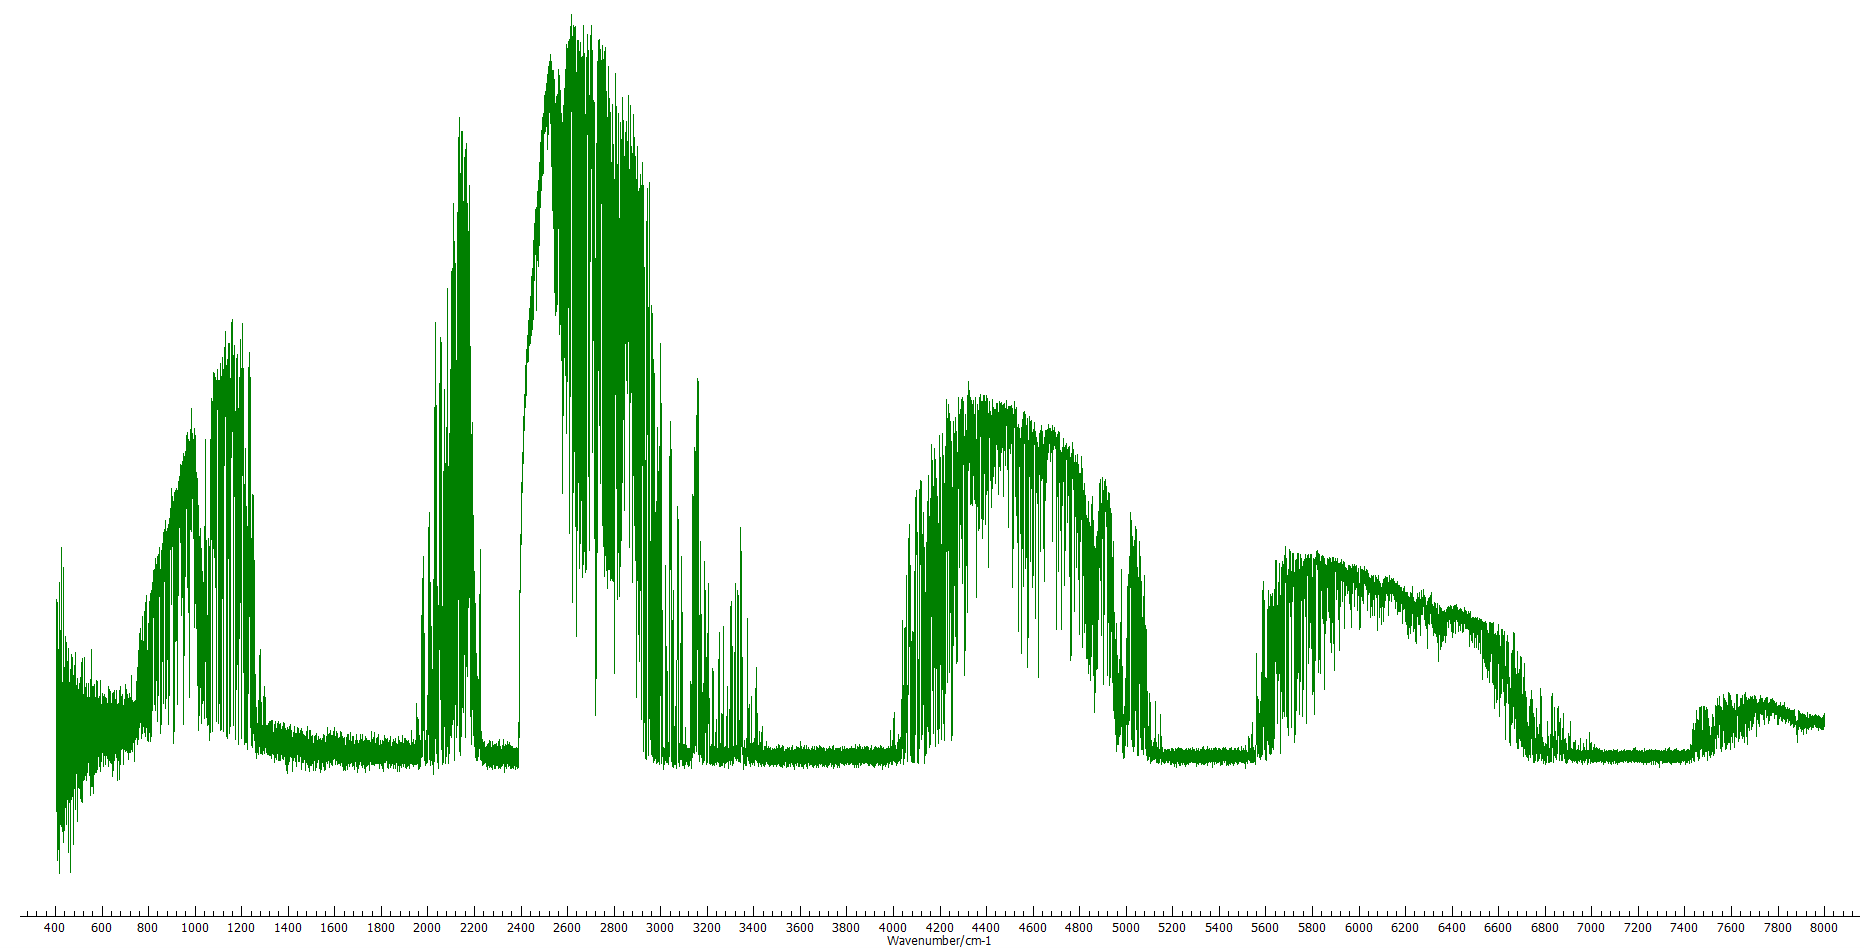
\includegraphics [width=0.80\textwidth] {SunSpectra.png} 
    \caption [Sun Spectra] {Absorption spectra of the sun with dense regions of absorption bands.}
    \label{fig: SunSpectra}
\end{figure}

The spectrum of sun is very wide compared to the other two, spanning from 300 $cm^{-1}$ to 8000 $cm^{-1}$. 
This gives us limited comparison of the spectra. We managed to identify 3 most prominent absorption bands. 
In the figure \ref{fig: Molecular_Regions} we have identified the corresponding molecules responsible for the absorption 
bands. The most prominent is water. Because of it's V-shaped structure it has many vibrational modes. Which are 
$3N - 6$ for non-linear molecules. Because of 3 fundamental vibrations, $H_2O$ has no clear P and R branches compared 
to $CO_2$. Which is second molecule we found. The visible P and R branches are result of the linear structure of $CO_2$.

\begin{figure} [H]
    \centering
    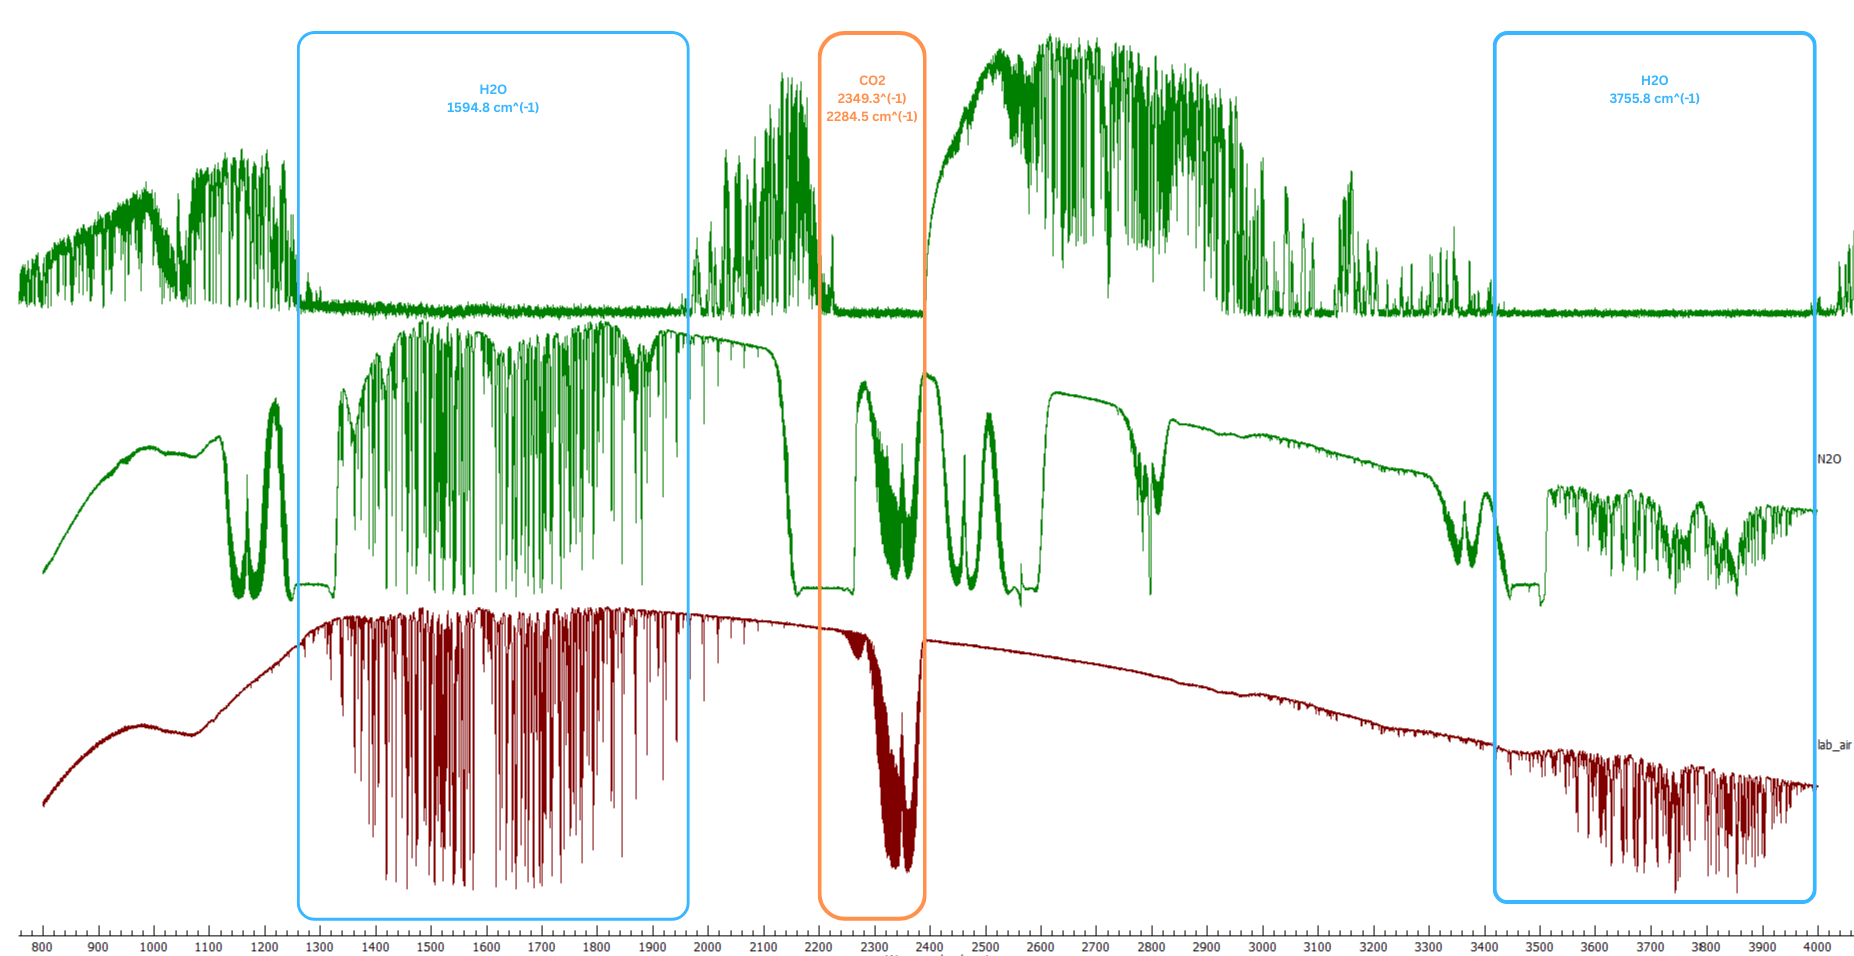
\includegraphics [width=0.80\textwidth] {Molecular_Regions.png} 
    \caption [Molecular Regions Highlighted] {This is the comparison of the spectra of sun(top), $N_2O$, and lab air
    , showing absorption bands. }
    \label{fig: Molecular_Regions}
\end{figure}

\subsection{Blackbody Temperature} \label{Subsec: BlackBody}

With the help of intensity maximum of the sun spectra we can calculate the temperature of the sun. Which is given by the
Wien's displacement law:

\begin{equation}
    \lambda_{\text{max}} = \frac{b}{T}
\end{equation}

with $b = 0.29 cm\cdot K$.

With the maximum of the spectrum at $2615.67 cm^{-1}$, the temperature of the sun came out to be $758.54 K$.
This is much lower than actual temperature of the sun which is around $5772 K$. This is because of the reasons
mentioned in the previous section \ref{Subsec: Spectra}.

In addition to that we also calculated the temperature of the lab air and $N_2O$ using the same method. 
The temperatures came out to be $527.69 K$ and $415.2 K$. This again is lower than the actual temperature of the
laser used for the experiment which is around $1000 K$. For this the reason is most likely the sensitivity of the instrument.

\subsection{Identification of the molecules}\label{Subsec: molecules}

By closely examining the solar spectra we found lot of absorption bands with P and R branches. The results are listed in a table
\ref{tab: Band Origins}

\begin{table}[ht]
\centering

\begin{tabular}{c | c | c}
\textbf{Observed Band Origin} (\si{cm^{-1}}) & \textbf{Literature Value} (\si{cm^{-1}}) & \textbf{Identified Molecule} \\
\hline
2462.6 & 2461.5 & N$_2$O \\
2563.3 & 2563.5 & N$_2$O \\
4855.5 & 4860.5 & CO$_2$ \\
4977.8 & 4983.5 & CO$_2$ \\
6228.4 & 6231.0 & CO$_2$ \\
6345.8 & 6351.0 & CO$_2$ \\
\end{tabular}

\caption[Band Origins and Literature Values]{Observed and Literature Band Origins of Atmospheric Trace Gases}
\label{tab: Band Origins}
\end{table}

Apart from the usual candidates we also found the absorption band near $1044.3 cm^{-1}$. This band was too hard to ignore with a prominent 
P and R branch see figure:\ref{fig: Ozone} As for what molecule this band is from, We are not sure. Only molecule with strong band at this
wavenumber is ozone. But ozone is not linear and hence should not have such clear P and R branches.
In literature we see the band of ozone at $1042 cm^{-1}$ \cite{amt-7-609-2014}. This is close to our observation but we are not sure.

\begin{figure} [H]
    \centering
    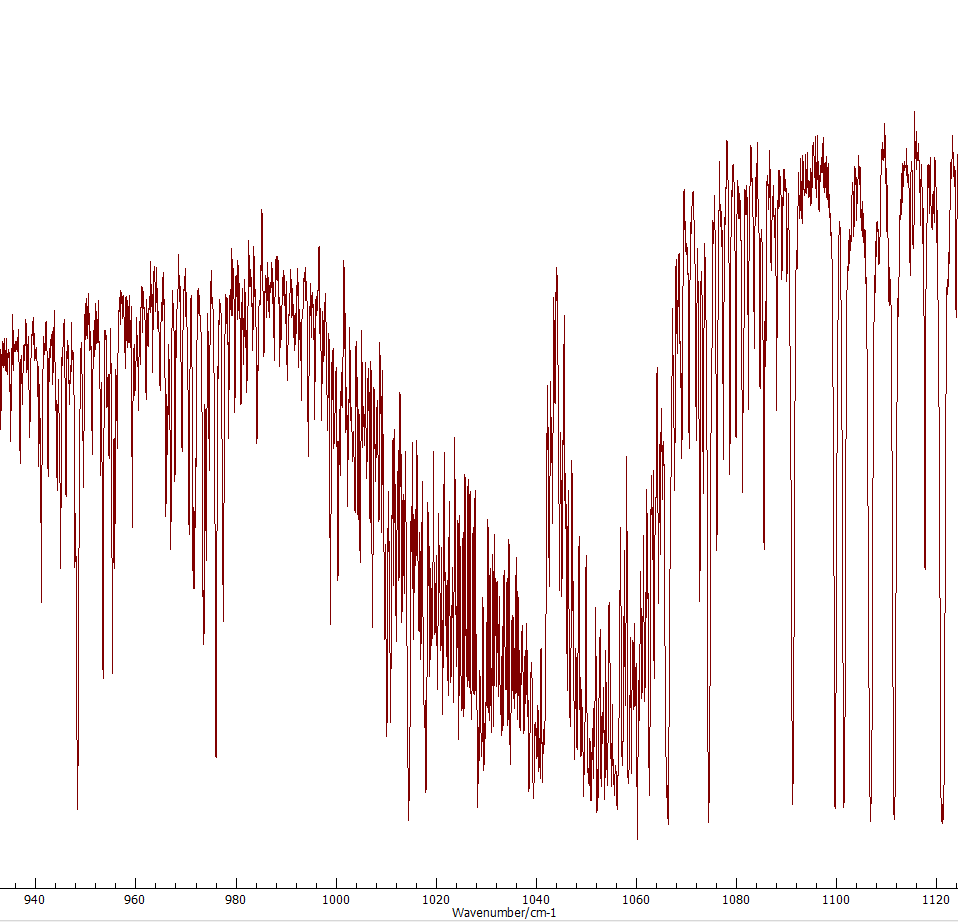
\includegraphics [width=0.60\textwidth] {Ozone.png} 
    \caption [Absorption Band] {Absorption band of with P and R branches.}
    \label{fig: Ozone}
\end{figure}

\subsection{Calculation of Moment of Inertia}\label{Subsec: MOI}

There is a lot of information that can be obtained from the spectra. With the spectra of $N_2O$ we
can calculate the moment of inertia of the molecule. The relation of the moment of inertia and the rotational
constant, $B$. This is stated in equation:\ref{equation: MOI}.

With the spectra of $N_20$ we select a band with clear P and R branches. We choose the band in the region
$1168.8 cm^{-1}$ shown in figure \ref{fig: N2O_Band}. We then note the distance between 5 consecutive lines.
The averaged distance is then $2B$. 

\begin{figure} [H]
    \centering
    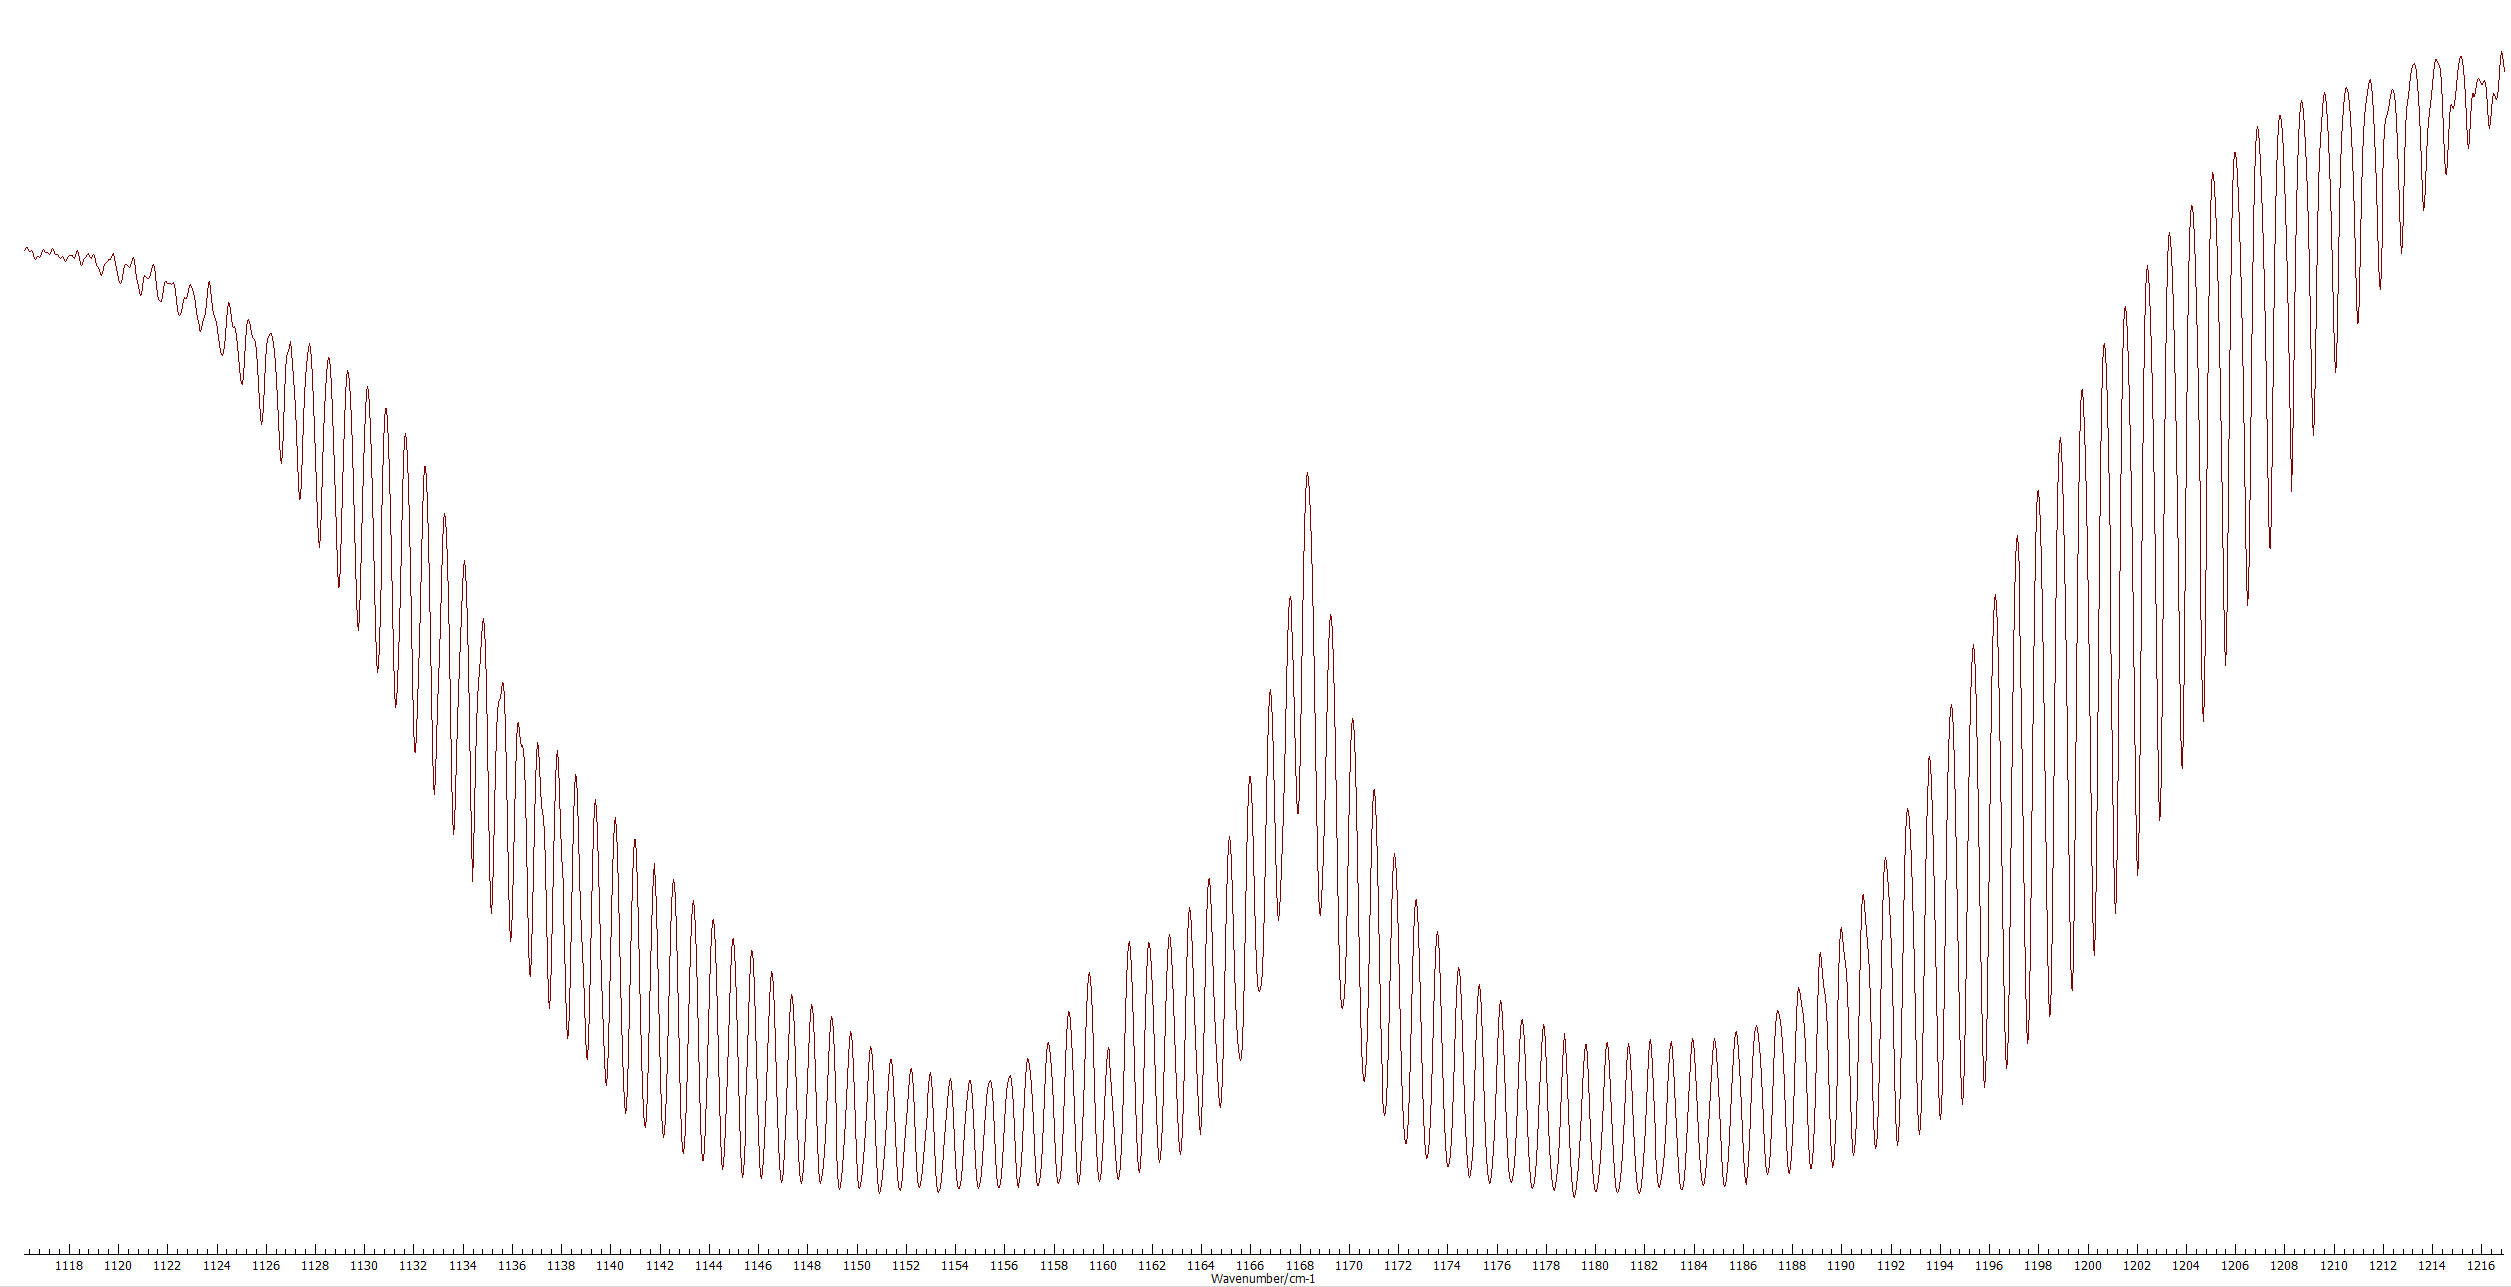
\includegraphics [width=0.60\textwidth] {N2OBand3.png} 
    \caption [Absorption Band of $N_2O$] {$N_2O$ Absorption bands chosen for moment of inertia calculation.}
    \label{fig: N2O_Band}
\end{figure}

The moment of inertia for $N_2O$ from the spectra came out to be $6.689 \times 10^{-47} kg \cdot m^2$. 
The literature value of the moment of inertia is $6.680 \times 10^{-47} kg \cdot m^2$. 
This is very close to our calculated value. The error is $0.13\%$.

\subsection {Determination of the gas pressure}\label{Subsec: Pressure}

For the pressure in the gas cell we used Lamber-Beer Law. The relation is already discussed in the 
section \ref{Subsec: LambertBeer}. With the help of absorption line strength, $S$, we can calculate 
the pressure with the following equation:

\begin{equation}
ln\left(\frac{I}{I_0}\right) = -S \cdot p \cdot L \cdot \frac{1}{\Delta \nu}
\end{equation}

$L = 15 \si{cm}$ is the length of the cell, $p$ is the quantity of interest, which is pressure and $S$ is the
band strength of the absorption line, for the particular line it was $\SI{10.9}{cm^{-2}.atm^{-1}}$. 

For the left side, $I$ is the intensity of the absorption line. and $I_0$ is the area under the curve of 
absorption line. After the relevant calculations we found the pressure of the gas sample inside the cell 
to be $\SI{0.4161}{atm}$.

\begin{figure} [H]
    \centering
    \includegraphics [width=0.60\textwidth] {N2O_band_Integration.png} 
    \caption [Absorption Band of $N_2O$] {$N_2O$ Absorption bands chosen for gas pressure calculation.}
    \label{fig: N2O_Band_Integration}
\end{figure}

\subsection{Temperature determination $N_2O$} \label{Subsec: Temperature}

To determine the temperature of the gas sample we used the relation already discussed in the section 
\ref{Subsec: IntensityDistribution}. The relation is \ref{equation:Temperature of gas}.

To determine the temperature we need to find the $J_{max}$. This is the number of lines from the center to the 
the maximum absorption line. We determined the $J_{max}$ from two different absorption bands. 

\begin{figure} [H]
    \centering
    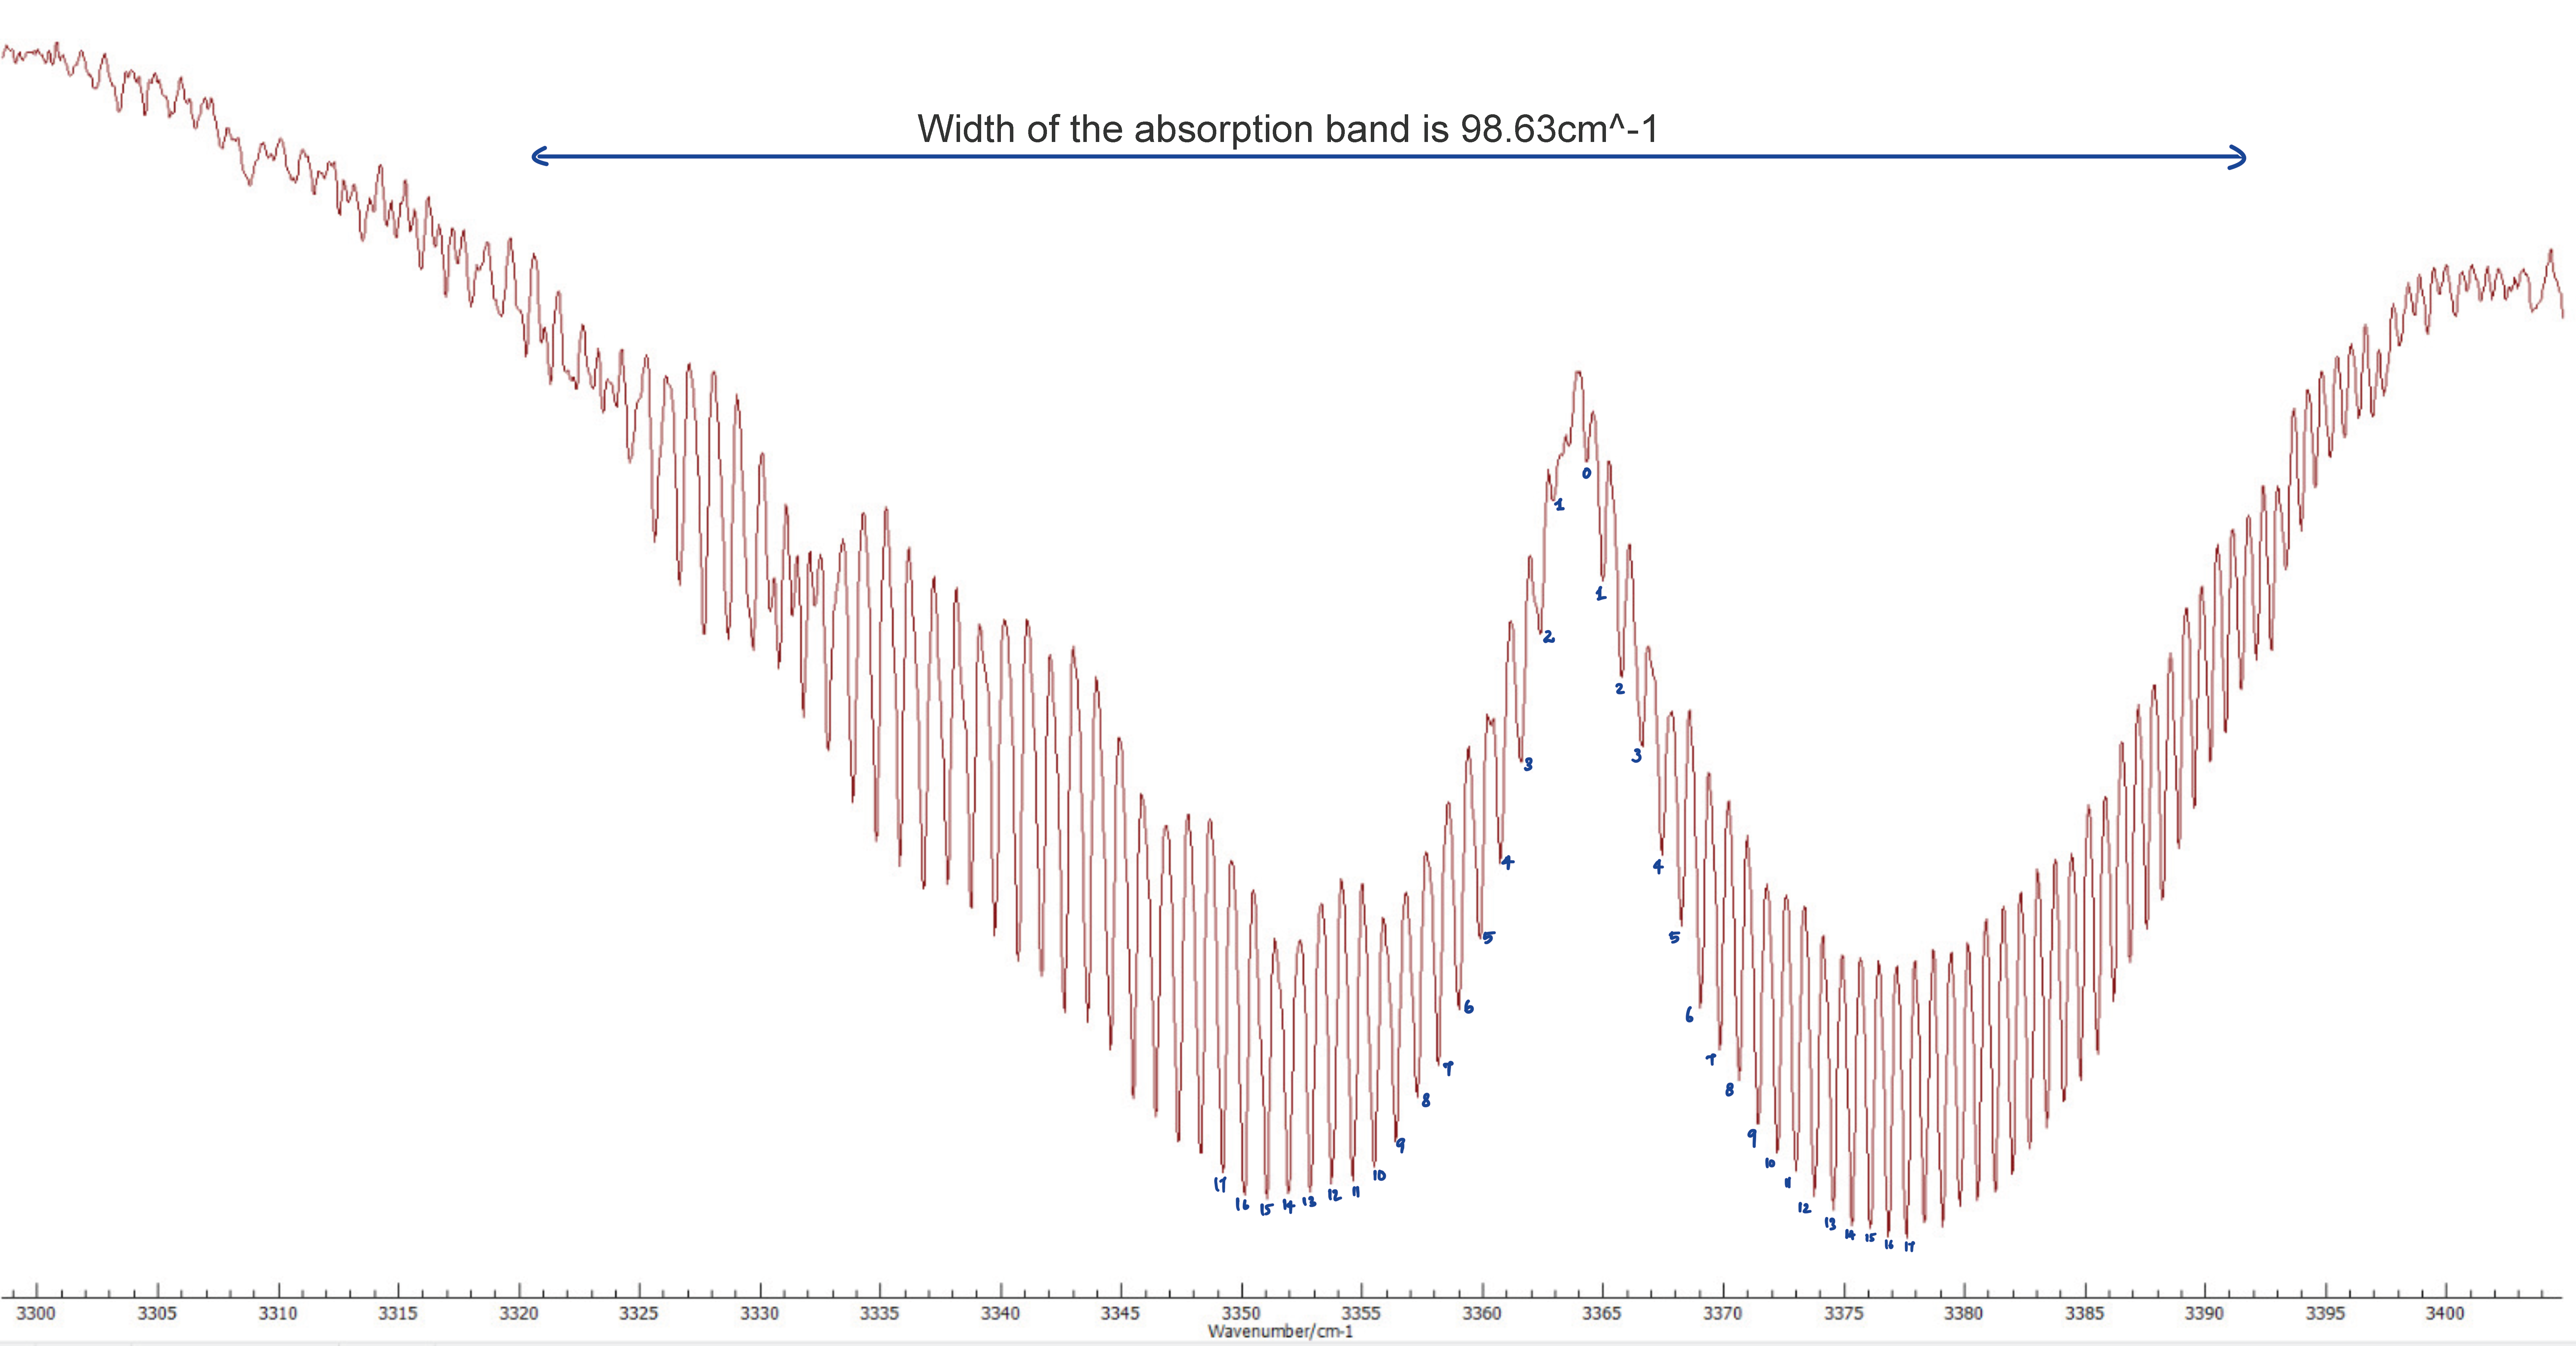
\includegraphics [width=0.80\textwidth] {N2OBand1.png} 
    \caption [Absorption Band of $N_2O$ with $J_{max}$]{$N_2O$ absorption band with $J_{max}$.}
    \label{fig: N2OBand2}
\end{figure}

With $J_max$ determined we can calculate the temperature of the gas in the cylinder. For the first 
band the the temperature came out to be $\SI{289.769}{K}$. And for the second absorption band, the temperature
was $\SI{328.364}{K}$.


\begin{figure} [H]
    \centering
    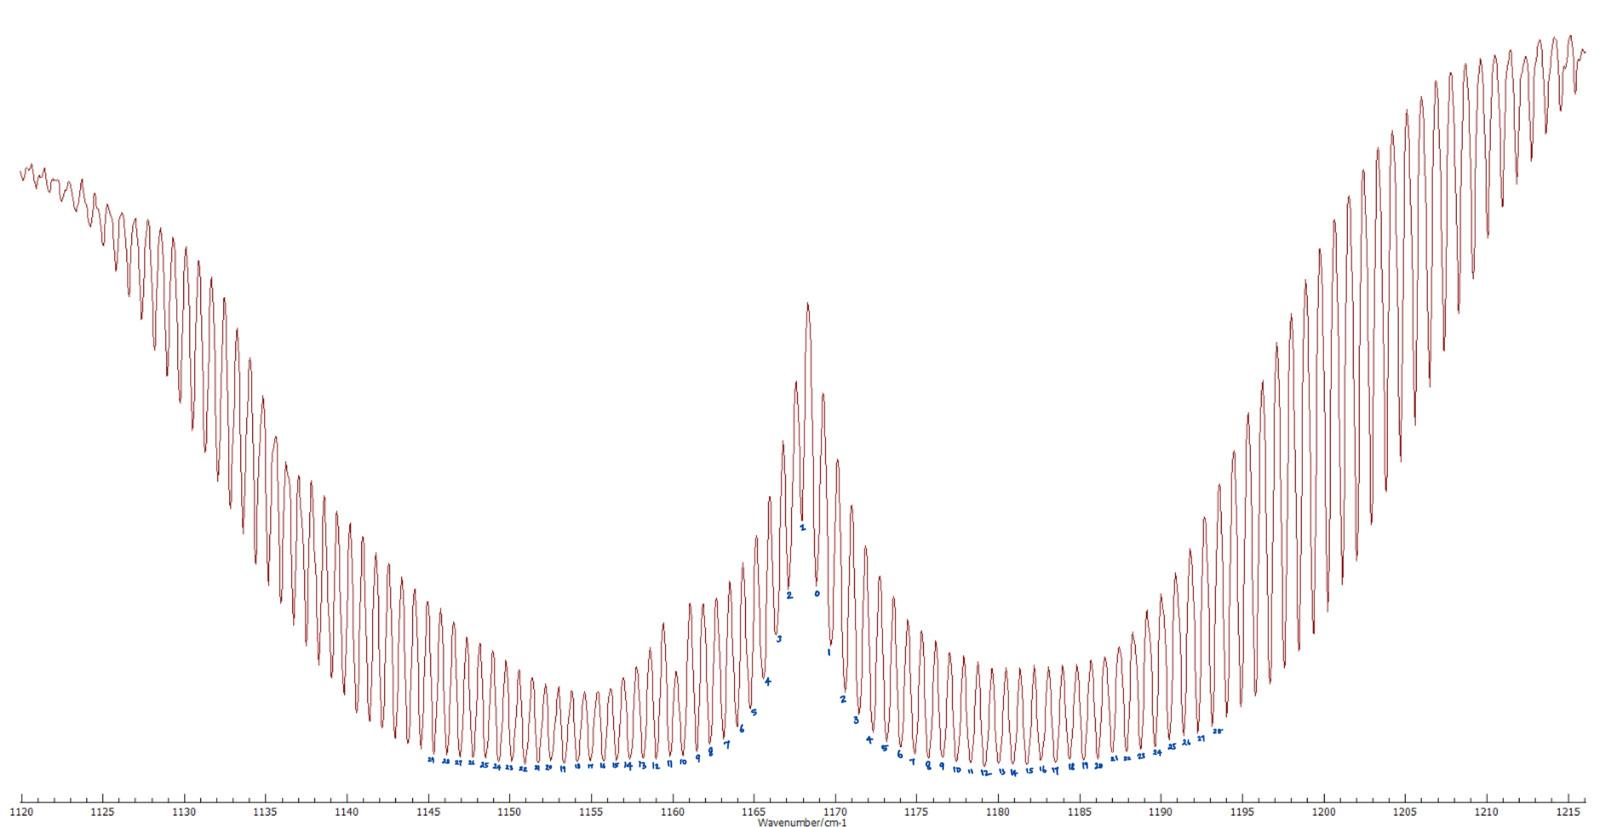
\includegraphics [width=0.80\textwidth] {N2OBand4.jpeg} 
    \caption [Absorption Band of $N_2O$ with $J_{max}$]{$N_2O$ absorption band with $J_{max}$.}
    \label{fig: N2OBand1}
\end{figure}



\subsection{Determination of the concentration of greenhouse gases}\label{Subsec: Concentration of greenhouse gases}

To determine the concentration of particular gas in the atmosphere we have to calculate the total number of molecules
in the atmosphere. To do that we will use the ideal gas law \ref{Equation: Ideal Gas Law}. With the pressure and 
temperature at the sea level we can estimate the number of particle at the sea level and then extrapolate the number
according to the pressure decrease with altitude. We will use the barometric altitude formula \ref{equation: Pressure with altitude}.

With this conditions the number of particle with altitude scales like shown in figure \ref{fig: Particle Density with Altitude}


\begin{figure} [H]
    \centering
    
\includegraphics [width=0.80\textwidth] {Particle_density.png} 
    \caption {Particle density vs. Altitude}
    \label{fig: Particle Density with Altitude}
\end{figure}


With particles at different altitudes we can integrate and get the number of particles in
a column, so called column density, $N_0$ which came out to be $\SI{1.619} \times {10^{25}}{cm^{-1}}$. 
For the total number of particle irradiated by the sun, we need to calculate the path length of light 
through the atmosphere. That depends on the inclination of the sun. For the provided spectra it was
$\SI{59}{\degree}$. The number of particle irradiated by the light is then calculated,

\begin{equation}
N_{ges} = \frac{N_0}{sin\alpha} = 2.5428 \times 10^{25}
\end{equation}

Now with the estimate of the total number of the particles in the atmosphere we can have the estimate
of the number of particular molecules in the atmosphere. For that we will again use the Lambert-Beer law,
in the form \ref{Equation: Lambert-Beer Law - coloumn form}. 

For $I_0$ (Irradiated Intensity), We will integrate with the linear baseline. Which is illustrated in the
\ref{} for $N_2O$ and \ref{} for $CO_2$. $I$ is the absorption intensity. 

\begin






